\documentclass[]{article}
\usepackage{lmodern}
\usepackage{amssymb,amsmath}
\usepackage{ifxetex,ifluatex}
\usepackage{fixltx2e} % provides \textsubscript
\ifnum 0\ifxetex 1\fi\ifluatex 1\fi=0 % if pdftex
  \usepackage[T1]{fontenc}
  \usepackage[utf8]{inputenc}
\else % if luatex or xelatex
  \ifxetex
    \usepackage{mathspec}
  \else
    \usepackage{fontspec}
  \fi
  \defaultfontfeatures{Ligatures=TeX,Scale=MatchLowercase}
\fi
% use upquote if available, for straight quotes in verbatim environments
\IfFileExists{upquote.sty}{\usepackage{upquote}}{}
% use microtype if available
\IfFileExists{microtype.sty}{%
\usepackage{microtype}
\UseMicrotypeSet[protrusion]{basicmath} % disable protrusion for tt fonts
}{}
\usepackage[margin=1in]{geometry}
\usepackage{hyperref}
\hypersetup{unicode=true,
            pdftitle={Homework 1},
            pdfauthor={PSTAT 131/231, Winter 2019},
            pdfborder={0 0 0},
            breaklinks=true}
\urlstyle{same}  % don't use monospace font for urls
\usepackage{color}
\usepackage{fancyvrb}
\newcommand{\VerbBar}{|}
\newcommand{\VERB}{\Verb[commandchars=\\\{\}]}
\DefineVerbatimEnvironment{Highlighting}{Verbatim}{commandchars=\\\{\}}
% Add ',fontsize=\small' for more characters per line
\usepackage{framed}
\definecolor{shadecolor}{RGB}{248,248,248}
\newenvironment{Shaded}{\begin{snugshade}}{\end{snugshade}}
\newcommand{\KeywordTok}[1]{\textcolor[rgb]{0.13,0.29,0.53}{\textbf{#1}}}
\newcommand{\DataTypeTok}[1]{\textcolor[rgb]{0.13,0.29,0.53}{#1}}
\newcommand{\DecValTok}[1]{\textcolor[rgb]{0.00,0.00,0.81}{#1}}
\newcommand{\BaseNTok}[1]{\textcolor[rgb]{0.00,0.00,0.81}{#1}}
\newcommand{\FloatTok}[1]{\textcolor[rgb]{0.00,0.00,0.81}{#1}}
\newcommand{\ConstantTok}[1]{\textcolor[rgb]{0.00,0.00,0.00}{#1}}
\newcommand{\CharTok}[1]{\textcolor[rgb]{0.31,0.60,0.02}{#1}}
\newcommand{\SpecialCharTok}[1]{\textcolor[rgb]{0.00,0.00,0.00}{#1}}
\newcommand{\StringTok}[1]{\textcolor[rgb]{0.31,0.60,0.02}{#1}}
\newcommand{\VerbatimStringTok}[1]{\textcolor[rgb]{0.31,0.60,0.02}{#1}}
\newcommand{\SpecialStringTok}[1]{\textcolor[rgb]{0.31,0.60,0.02}{#1}}
\newcommand{\ImportTok}[1]{#1}
\newcommand{\CommentTok}[1]{\textcolor[rgb]{0.56,0.35,0.01}{\textit{#1}}}
\newcommand{\DocumentationTok}[1]{\textcolor[rgb]{0.56,0.35,0.01}{\textbf{\textit{#1}}}}
\newcommand{\AnnotationTok}[1]{\textcolor[rgb]{0.56,0.35,0.01}{\textbf{\textit{#1}}}}
\newcommand{\CommentVarTok}[1]{\textcolor[rgb]{0.56,0.35,0.01}{\textbf{\textit{#1}}}}
\newcommand{\OtherTok}[1]{\textcolor[rgb]{0.56,0.35,0.01}{#1}}
\newcommand{\FunctionTok}[1]{\textcolor[rgb]{0.00,0.00,0.00}{#1}}
\newcommand{\VariableTok}[1]{\textcolor[rgb]{0.00,0.00,0.00}{#1}}
\newcommand{\ControlFlowTok}[1]{\textcolor[rgb]{0.13,0.29,0.53}{\textbf{#1}}}
\newcommand{\OperatorTok}[1]{\textcolor[rgb]{0.81,0.36,0.00}{\textbf{#1}}}
\newcommand{\BuiltInTok}[1]{#1}
\newcommand{\ExtensionTok}[1]{#1}
\newcommand{\PreprocessorTok}[1]{\textcolor[rgb]{0.56,0.35,0.01}{\textit{#1}}}
\newcommand{\AttributeTok}[1]{\textcolor[rgb]{0.77,0.63,0.00}{#1}}
\newcommand{\RegionMarkerTok}[1]{#1}
\newcommand{\InformationTok}[1]{\textcolor[rgb]{0.56,0.35,0.01}{\textbf{\textit{#1}}}}
\newcommand{\WarningTok}[1]{\textcolor[rgb]{0.56,0.35,0.01}{\textbf{\textit{#1}}}}
\newcommand{\AlertTok}[1]{\textcolor[rgb]{0.94,0.16,0.16}{#1}}
\newcommand{\ErrorTok}[1]{\textcolor[rgb]{0.64,0.00,0.00}{\textbf{#1}}}
\newcommand{\NormalTok}[1]{#1}
\usepackage{graphicx,grffile}
\makeatletter
\def\maxwidth{\ifdim\Gin@nat@width>\linewidth\linewidth\else\Gin@nat@width\fi}
\def\maxheight{\ifdim\Gin@nat@height>\textheight\textheight\else\Gin@nat@height\fi}
\makeatother
% Scale images if necessary, so that they will not overflow the page
% margins by default, and it is still possible to overwrite the defaults
% using explicit options in \includegraphics[width, height, ...]{}
\setkeys{Gin}{width=\maxwidth,height=\maxheight,keepaspectratio}
\IfFileExists{parskip.sty}{%
\usepackage{parskip}
}{% else
\setlength{\parindent}{0pt}
\setlength{\parskip}{6pt plus 2pt minus 1pt}
}
\setlength{\emergencystretch}{3em}  % prevent overfull lines
\providecommand{\tightlist}{%
  \setlength{\itemsep}{0pt}\setlength{\parskip}{0pt}}
\setcounter{secnumdepth}{0}
% Redefines (sub)paragraphs to behave more like sections
\ifx\paragraph\undefined\else
\let\oldparagraph\paragraph
\renewcommand{\paragraph}[1]{\oldparagraph{#1}\mbox{}}
\fi
\ifx\subparagraph\undefined\else
\let\oldsubparagraph\subparagraph
\renewcommand{\subparagraph}[1]{\oldsubparagraph{#1}\mbox{}}
\fi

%%% Use protect on footnotes to avoid problems with footnotes in titles
\let\rmarkdownfootnote\footnote%
\def\footnote{\protect\rmarkdownfootnote}

%%% Change title format to be more compact
\usepackage{titling}

% Create subtitle command for use in maketitle
\newcommand{\subtitle}[1]{
  \posttitle{
    \begin{center}\large#1\end{center}
    }
}

\setlength{\droptitle}{-2em}

  \title{Homework 1}
    \pretitle{\vspace{\droptitle}\centering\huge}
  \posttitle{\par}
    \author{PSTAT 131/231, Winter 2019}
    \preauthor{\centering\large\emph}
  \postauthor{\par}
      \predate{\centering\large\emph}
  \postdate{\par}
    \date{\textbf{Due on January 26, 2018 at 11:55 pm}}

\usepackage{booktabs}
\usepackage{longtable}
\usepackage{array}
\usepackage{multirow}
\usepackage[table]{xcolor}
\usepackage{wrapfig}
\usepackage{float}
\usepackage{colortbl}
\usepackage{pdflscape}
\usepackage{tabu}
\usepackage{threeparttable}
\usepackage{threeparttablex}
\usepackage[normalem]{ulem}
\usepackage{makecell}

\begin{document}
\maketitle

\textbf{Note:} If you are working with a partner, please submit only one
homework per group with both names and whether you are taking the course
for graduate credit or not. Submit your Rmarkdown (.Rmd) and the
compiled pdf on Gauchospace.

\begin{center}\rule{0.5\linewidth}{\linethickness}\end{center}

\textbf{Predicting Algae Blooms}

\textbf{\emph{Background}} High concentrations of certain harmful algae
in rivers constitute a serious ecological problem with a strong impact
not only on river lifeforms, but also on water quality. Being able to
monitor and perform an early forecast of algae blooms is essential to
improving the quality of rivers.

With the goal of addressing this prediction problem, several water
samples were collected in different European rivers at different times
during a period of approximately 1 year. For each water sample,
different chemical properties were measured as well as the frequency of
occurrence of seven harmful algae. Some other characteristics of the
water collection process were also stored, such as the season of the
year, the river size, and the river speed.

\textbf{\emph{Goal}} We want to understand how these frequencies are
related to certain chemical attributes of water samples as well as other
characteristics of the samples (like season of the year, type of river,
etc.)

\textbf{\emph{Data Description}} The data set consists of data for 200
water samples and each observation in the available datasets is in
effect an aggregation of several water samples collected from the same
river over a period of 3 months, during the same season of the year.
Each observation contains information on 11 variables. Three of these
variables are nominal and describe the season of the year when the water
samples to be aggregated were collected, as well as the size and speed
of the river in question. The eight remaining variables are values of
different chemical parameters measured in the water samples forming the
aggregation, namely: Maximum pH value, Minimum value of \(O_2\)
(oxygen), Mean value of Cl (chloride), Mean value of \(NO_3^-\)
(nitrates), Mean value of \(NH_4^+\) (ammonium), Mean of \(PO^{3}_4\)
(orthophosphate), Mean of total \(PO_4\) (phosphate) and Mean of
chlorophyll.

Associated with each of these parameters are seven frequency numbers of
different harmful algae found in the respective water samples. No
information is given regarding the names of the algae that were
identified.

We can start the analysis by loading into R the data from the
``algaeBloom.txt'' file (the training data, i.e.~the data that will be
used to obtain the predictive models). To read the data from the file it
is sufficient to issue the following command:

\begin{Shaded}
\begin{Highlighting}[]
\NormalTok{algae <-}\StringTok{ }\KeywordTok{read_table2}\NormalTok{(}\StringTok{"algaeBloom.txt"}\NormalTok{, }\DataTypeTok{col_names=}
                      \KeywordTok{c}\NormalTok{(}\StringTok{'season'}\NormalTok{,}\StringTok{'size'}\NormalTok{,}\StringTok{'speed'}\NormalTok{,}\StringTok{'mxPH'}\NormalTok{,}\StringTok{'mnO2'}\NormalTok{,}\StringTok{'Cl'}\NormalTok{,}\StringTok{'NO3'}\NormalTok{,}\StringTok{'NH4'}\NormalTok{,}
                        \StringTok{'oPO4'}\NormalTok{,}\StringTok{'PO4'}\NormalTok{,}\StringTok{'Chla'}\NormalTok{,}\StringTok{'a1'}\NormalTok{,}\StringTok{'a2'}\NormalTok{,}\StringTok{'a3'}\NormalTok{,}\StringTok{'a4'}\NormalTok{,}\StringTok{'a5'}\NormalTok{,}\StringTok{'a6'}\NormalTok{,}\StringTok{'a7'}\NormalTok{), }
                      \DataTypeTok{na=}\StringTok{"XXXXXXX"}\NormalTok{)}

\KeywordTok{glimpse}\NormalTok{(algae)}
\end{Highlighting}
\end{Shaded}

\begin{enumerate}
\def\labelenumi{\arabic{enumi}.}
\item
  \textbf{\emph{Descriptive summary statistics}} Given the lack of
  further information on the problem domain, it is wise to investigate
  some of the statistical properties of the data, so as to get a better
  grasp of the problem. It is always a good idea to start our analysis
  with some kind of exploratory data analysis. A first idea of the
  statistical properties of the data can be obtained through a summary
  of its descriptive statistics.

  \begin{enumerate}
  \tightlist
  \item
    Count the number of observations in each season using
    \texttt{summarise()} in \texttt{dplyr}.
  \end{enumerate}
\end{enumerate}

\begin{Shaded}
\begin{Highlighting}[]
\NormalTok{season_obs <-}\StringTok{ }\NormalTok{algae }\OperatorTok\StringTok{ }
\StringTok{  }\KeywordTok{group_by}\NormalTok{(season) }\OperatorTok\StringTok{ }
\StringTok{  }\KeywordTok{summarize}\NormalTok{(}\DataTypeTok{obs_count =} \KeywordTok{n}\NormalTok{())}
\end{Highlighting}
\end{Shaded}

\begin{verbatim}
#. Are there missing values? Calculate the mean and variance of each
chemical (Ignore $a_1$ through $a_7$). What do you notice about the
magnitude of the two quantities for different chemicals? 
\end{verbatim}

\begin{Shaded}
\begin{Highlighting}[]
\NormalTok{algae_na <-}\StringTok{ }\NormalTok{algae }\OperatorTok
\StringTok{  }\KeywordTok{select}\NormalTok{(}\KeywordTok{c}\NormalTok{(}\StringTok{'mxPH'}\NormalTok{,}\StringTok{'mnO2'}\NormalTok{,}\StringTok{'Cl'}\NormalTok{,}\StringTok{'NO3'}\NormalTok{,}\StringTok{'NH4'}\NormalTok{, }\StringTok{'oPO4'}\NormalTok{,}\StringTok{'PO4'}\NormalTok{,}\StringTok{'Chla'}\NormalTok{)) }\OperatorTok
\StringTok{  }\KeywordTok{summarise_all}\NormalTok{(}\ControlFlowTok{function}\NormalTok{(x) }\KeywordTok{sum}\NormalTok{(}\KeywordTok{is.na}\NormalTok{(x)))}
\end{Highlighting}
\end{Shaded}

There are missing values for several variables. One value is missing for
mxPH. NO3, NH4, oPO4, and PO4 are all missing two values. Cl and Chla
are each missing 10 and 12 variables.

\begin{Shaded}
\begin{Highlighting}[]
\KeywordTok{print}\NormalTok{(}\StringTok{'Mean'}\NormalTok{)}
\end{Highlighting}
\end{Shaded}

\begin{verbatim}
## [1] "Mean"
\end{verbatim}

\begin{Shaded}
\begin{Highlighting}[]
\NormalTok{chem_means <-}\StringTok{ }\NormalTok{algae }\OperatorTok\StringTok{ }
\StringTok{  }\KeywordTok{select}\NormalTok{(}\KeywordTok{c}\NormalTok{(}\StringTok{'mxPH'}\NormalTok{,}\StringTok{'mnO2'}\NormalTok{,}\StringTok{'Cl'}\NormalTok{,}\StringTok{'NO3'}\NormalTok{,}\StringTok{'NH4'}\NormalTok{, }\StringTok{'oPO4'}\NormalTok{,}\StringTok{'PO4'}\NormalTok{,}\StringTok{'Chla'}\NormalTok{)) }\OperatorTok
\StringTok{  }\KeywordTok{summarise_all}\NormalTok{(}\ControlFlowTok{function}\NormalTok{ (x) }\KeywordTok{mean}\NormalTok{(x, }\DataTypeTok{na.rm=}\OtherTok{TRUE}\NormalTok{)) }

\KeywordTok{print}\NormalTok{(}\StringTok{'Variance'}\NormalTok{)}
\end{Highlighting}
\end{Shaded}

\begin{verbatim}
## [1] "Variance"
\end{verbatim}

\begin{Shaded}
\begin{Highlighting}[]
\NormalTok{chem_vars <-}\StringTok{ }\NormalTok{algae }\OperatorTok\StringTok{ }
\StringTok{   }\KeywordTok{select}\NormalTok{(}\KeywordTok{c}\NormalTok{(}\StringTok{'mxPH'}\NormalTok{,}\StringTok{'mnO2'}\NormalTok{,}\StringTok{'Cl'}\NormalTok{,}\StringTok{'NO3'}\NormalTok{,}\StringTok{'NH4'}\NormalTok{, }\StringTok{'oPO4'}\NormalTok{,}\StringTok{'PO4'}\NormalTok{,}\StringTok{'Chla'}\NormalTok{)) }\OperatorTok
\StringTok{  }\KeywordTok{summarise_all}\NormalTok{(}\ControlFlowTok{function}\NormalTok{ (x) }\KeywordTok{var}\NormalTok{(x, }\DataTypeTok{na.rm=}\OtherTok{TRUE}\NormalTok{)) }
\end{Highlighting}
\end{Shaded}

The mean for NH4 is the largest, but it also has a disproportionately
large variance as compared to the mean and variance coupling of other
variables.

\begin{verbatim}
#. Mean and Variance is one measure of central tendency and spread of data.
Median and Median Absolute Deviation are alternative measures of central
tendency and spread. 

    For a univariate data set $X_1, X_2, ..., X_n$, the Median Absolute Deviation (MAD) is defined as the median of the absolute deviations from the data's median: $$\text{MAD}=\text{median} (|X_i-\text{median}(X)|)$$

    Compute median and MAD of each chemical and compare the two sets of quantities (i.e., mean & variance vs. median & MAD). What do you notice? 
    
\end{verbatim}

\begin{Shaded}
\begin{Highlighting}[]
\KeywordTok{print}\NormalTok{(}\StringTok{'Median'}\NormalTok{)}
\end{Highlighting}
\end{Shaded}

\begin{verbatim}
## [1] "Median"
\end{verbatim}

\begin{Shaded}
\begin{Highlighting}[]
\NormalTok{chem_medians <-}\StringTok{ }\NormalTok{algae }\OperatorTok\StringTok{ }
\StringTok{  }\KeywordTok{select}\NormalTok{(}\KeywordTok{c}\NormalTok{(}\StringTok{'mxPH'}\NormalTok{,}\StringTok{'mnO2'}\NormalTok{,}\StringTok{'Cl'}\NormalTok{,}\StringTok{'NO3'}\NormalTok{,}\StringTok{'NH4'}\NormalTok{, }\StringTok{'oPO4'}\NormalTok{,}\StringTok{'PO4'}\NormalTok{,}\StringTok{'Chla'}\NormalTok{)) }\OperatorTok\StringTok{ }
\StringTok{  }\KeywordTok{summarise_all}\NormalTok{(}\ControlFlowTok{function}\NormalTok{ (x) }\KeywordTok{median}\NormalTok{(x, }\DataTypeTok{na.rm=}\OtherTok{TRUE}\NormalTok{))}

\KeywordTok{print}\NormalTok{(}\StringTok{'MADs'}\NormalTok{)}
\end{Highlighting}
\end{Shaded}

\begin{verbatim}
## [1] "MADs"
\end{verbatim}

\begin{Shaded}
\begin{Highlighting}[]
\NormalTok{chem_mads <-}\StringTok{ }\NormalTok{algae }\OperatorTok\StringTok{ }
\StringTok{  }\KeywordTok{select}\NormalTok{(}\KeywordTok{c}\NormalTok{(}\StringTok{'mxPH'}\NormalTok{,}\StringTok{'mnO2'}\NormalTok{,}\StringTok{'Cl'}\NormalTok{,}\StringTok{'NO3'}\NormalTok{,}\StringTok{'NH4'}\NormalTok{, }\StringTok{'oPO4'}\NormalTok{,}\StringTok{'PO4'}\NormalTok{,}\StringTok{'Chla'}\NormalTok{)) }\OperatorTok
\StringTok{  }\KeywordTok{summarise_all}\NormalTok{(}\ControlFlowTok{function}\NormalTok{ (x) }\KeywordTok{mad}\NormalTok{(x, }\DataTypeTok{na.rm=}\OtherTok{TRUE}\NormalTok{))}
\end{Highlighting}
\end{Shaded}

\begin{enumerate}
\def\labelenumi{\arabic{enumi}.}
\setcounter{enumi}{1}
\item
  \textbf{\emph{Data visualization}} Most of the time, the information
  in the data set is also well captured graphically. Histogram, scatter
  plot, boxplot, Q-Q plot are frequently used tools for data
  visualization. Use ggplot for all of these visualizations.

  \begin{enumerate}
  \tightlist
  \item
    Produce a histogram of \(mxPH\) with the title `Histogram of mxPH'
    based on algae data set. Use an appropriate argument to show the
    probability instead of the frequency as the vertical axis. (Hint:
    look at the examples in the help file for function
    \texttt{geom\_histogram()}). Is the distribution skewed?
  \end{enumerate}
\end{enumerate}

\begin{Shaded}
\begin{Highlighting}[]
\NormalTok{hist_mxPH <-}\StringTok{ }\KeywordTok{ggplot}\NormalTok{(algae, }\KeywordTok{aes}\NormalTok{(}\DataTypeTok{x =}\NormalTok{ mxPH)) }\OperatorTok{+}
\StringTok{  }\KeywordTok{geom_histogram}\NormalTok{(}\DataTypeTok{bins =} \DecValTok{12}\NormalTok{)  }\OperatorTok{+}\StringTok{ }\CommentTok{#2*(200)^1/3}
\StringTok{  }\KeywordTok{labs}\NormalTok{(}\DataTypeTok{title =} \StringTok{'Histogram of mxPH'}\NormalTok{) }\OperatorTok{+}
\StringTok{  }\KeywordTok{ylab}\NormalTok{(}\StringTok{'Probability'}\NormalTok{) }\OperatorTok{+}
\StringTok{  }\KeywordTok{scale_y_continuous}\NormalTok{(}\DataTypeTok{labels =}\NormalTok{scales}\OperatorTok{::}\NormalTok{percent) }\OperatorTok{+}
\StringTok{  }\KeywordTok{geom_density}\NormalTok{() }\OperatorTok{+}
\StringTok{  }\KeywordTok{geom_rug}\NormalTok{()}

\NormalTok{hist_mxPH}
\end{Highlighting}
\end{Shaded}

\begin{verbatim}
## Warning: Removed 1 rows containing non-finite values (stat_bin).
\end{verbatim}

\begin{verbatim}
## Warning: Removed 1 rows containing non-finite values (stat_density).
\end{verbatim}

\begin{center}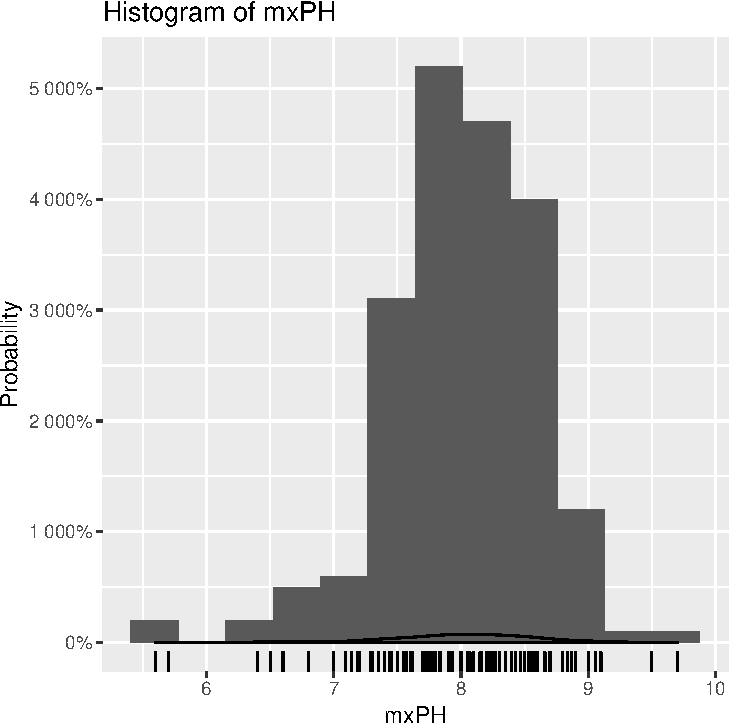
\includegraphics{homework1-handout_files/figure-latex/unnamed-chunk-1-1} \end{center}

\begin{enumerate}
\item
  Add a density curve using \texttt{geom\_density()} and rug plots using
  \texttt{geom\_rug()} to above histogram.

  \begin{enumerate}
  \tightlist
  \item
    Create a boxplot with the title `A conditioned Boxplot of Algal
    \(a_1\)' for \(a_1\) grouped by \(size\). (Refer to help page for
    \texttt{geom\_boxplot()}).
  \end{enumerate}
\end{enumerate}

\begin{Shaded}
\begin{Highlighting}[]
\NormalTok{algae_boxplot <-}\StringTok{ }\KeywordTok{ggplot}\NormalTok{(algae, }\KeywordTok{aes}\NormalTok{(size, a1)) }\OperatorTok{+}
\StringTok{  }\KeywordTok{geom_boxplot}\NormalTok{(}\DataTypeTok{outlier.color =} \StringTok{'orange'}\NormalTok{) }\OperatorTok{+}
\StringTok{  }\KeywordTok{labs}\NormalTok{(}\DataTypeTok{title =} \StringTok{'A conditioned Boxplot of Algal a1'}\NormalTok{)}

\NormalTok{algae_boxplot}
\end{Highlighting}
\end{Shaded}

\begin{center}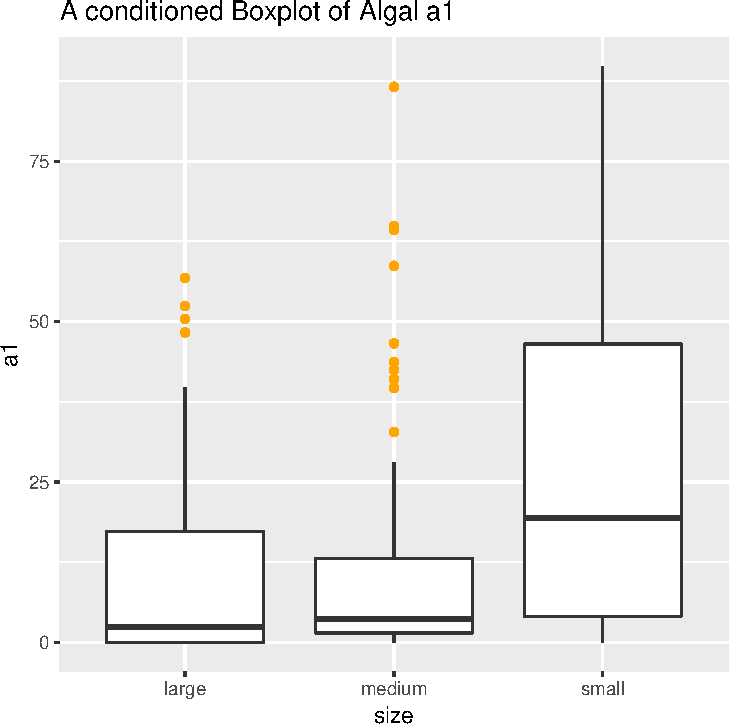
\includegraphics{homework1-handout_files/figure-latex/boxplot-1} \end{center}

\begin{enumerate}
\tightlist
\item
  Are there any outliers for \(NO3\) and \(NH4\)? How many observations
  would you consider as outliers? How did you arrive at this conclusion?
\end{enumerate}

\begin{Shaded}
\begin{Highlighting}[]
\NormalTok{NO3_boxplot <-}\StringTok{ }\KeywordTok{ggplot}\NormalTok{(algae, }\KeywordTok{aes}\NormalTok{(}\DataTypeTok{x =} \StringTok{'NO3'}\NormalTok{, }\DataTypeTok{y =}\NormalTok{ NO3)) }\OperatorTok{+}\StringTok{ }
\StringTok{  }\KeywordTok{geom_boxplot}\NormalTok{(}\DataTypeTok{outlier.color =} \StringTok{'orange'}\NormalTok{) }\OperatorTok{+}
\StringTok{  }\KeywordTok{labs}\NormalTok{(}\DataTypeTok{title =} \StringTok{'A conditioned Boxplot of NO3'}\NormalTok{)}

\NormalTok{NO3_boxplot }
\end{Highlighting}
\end{Shaded}

\begin{verbatim}
## Warning: Removed 2 rows containing non-finite values (stat_boxplot).
\end{verbatim}

\begin{center}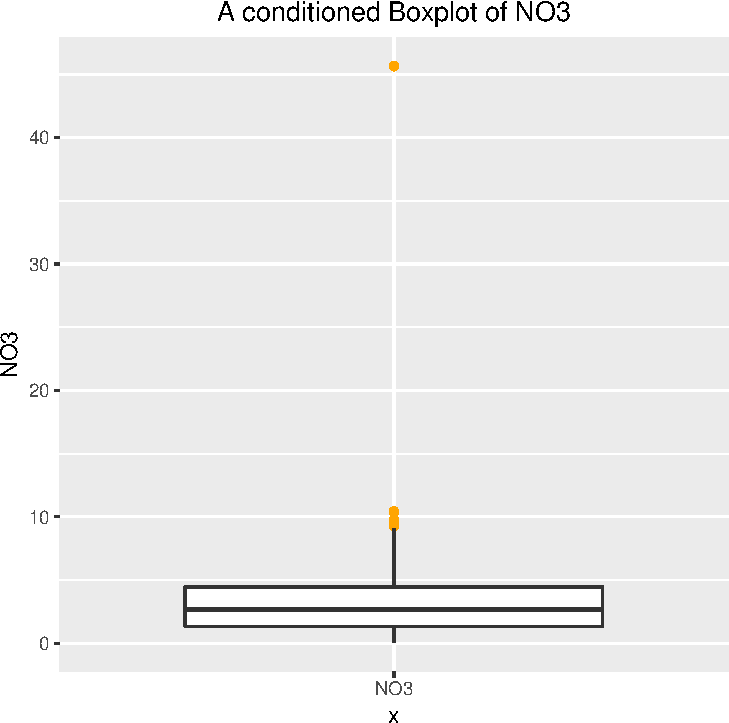
\includegraphics{homework1-handout_files/figure-latex/unnamed-chunk-2-1} \end{center}

\begin{Shaded}
\begin{Highlighting}[]
\NormalTok{NO3season_boxplot <-}\StringTok{ }\KeywordTok{ggplot}\NormalTok{(algae, }\KeywordTok{aes}\NormalTok{(season, }\DataTypeTok{y =}\NormalTok{ NO3)) }\OperatorTok{+}
\StringTok{  }\KeywordTok{geom_boxplot}\NormalTok{(}\DataTypeTok{outlier.color =} \StringTok{'orange'}\NormalTok{) }\OperatorTok{+}
\StringTok{  }\KeywordTok{labs}\NormalTok{(}\DataTypeTok{title =} \StringTok{'A conditioned Boxplot of NO3 by Season'}\NormalTok{)}

\NormalTok{NO3season_boxplot}
\end{Highlighting}
\end{Shaded}

\begin{verbatim}
## Warning: Removed 2 rows containing non-finite values (stat_boxplot).
\end{verbatim}

\begin{center}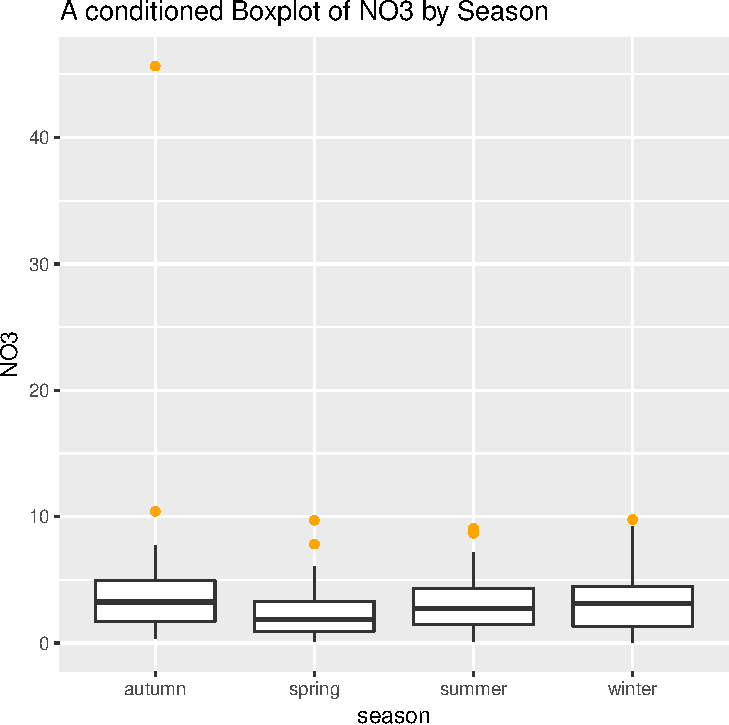
\includegraphics{homework1-handout_files/figure-latex/unnamed-chunk-2-2} \end{center}

By separating the NO3 data into seasons, we can see that there is a
clear outlier in autumn that is significantly further from the
Interquartile Range than outliers in other months. Note: outliers are
indicated in orange. Thus, we will only consider this one autumn outlier
as a true outlier.

\begin{Shaded}
\begin{Highlighting}[]
\NormalTok{NH4_boxplot <-}\StringTok{ }\KeywordTok{ggplot}\NormalTok{(algae, }\KeywordTok{aes}\NormalTok{(}\DataTypeTok{x =} \StringTok{'NH4'}\NormalTok{, }\DataTypeTok{y =}\NormalTok{ NH4)) }\OperatorTok{+}\StringTok{ }
\StringTok{  }\KeywordTok{geom_boxplot}\NormalTok{(}\DataTypeTok{outlier.color =} \StringTok{'orange'}\NormalTok{) }\OperatorTok{+}
\StringTok{  }\KeywordTok{labs}\NormalTok{(}\DataTypeTok{title =} \StringTok{'A conditioned Boxplot of NH4'}\NormalTok{)}

\NormalTok{NH4_boxplot }
\end{Highlighting}
\end{Shaded}

\begin{verbatim}
## Warning: Removed 2 rows containing non-finite values (stat_boxplot).
\end{verbatim}

\begin{center}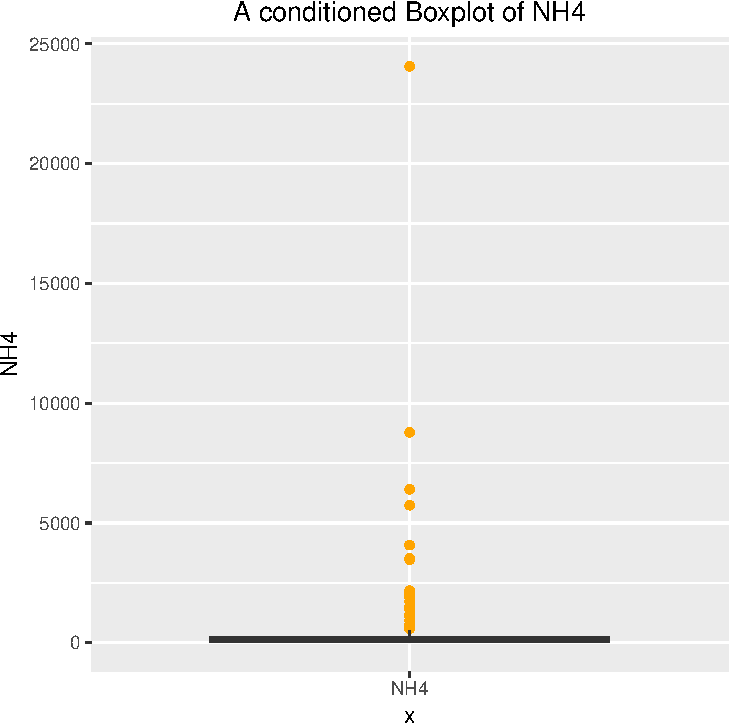
\includegraphics{homework1-handout_files/figure-latex/unnamed-chunk-3-1} \end{center}

\begin{Shaded}
\begin{Highlighting}[]
\NormalTok{NH4season_boxplot <-}\StringTok{ }\KeywordTok{ggplot}\NormalTok{(algae, }\KeywordTok{aes}\NormalTok{(season, }\DataTypeTok{y =}\NormalTok{ NH4)) }\OperatorTok{+}
\StringTok{  }\KeywordTok{geom_boxplot}\NormalTok{(}\DataTypeTok{outlier.color =} \StringTok{'orange'}\NormalTok{) }\OperatorTok{+}
\StringTok{  }\KeywordTok{labs}\NormalTok{(}\DataTypeTok{title =} \StringTok{'A conditioned Boxplot of NH4 by Season'}\NormalTok{)}

\NormalTok{NH4season_boxplot}
\end{Highlighting}
\end{Shaded}

\begin{verbatim}
## Warning: Removed 2 rows containing non-finite values (stat_boxplot).
\end{verbatim}

\begin{center}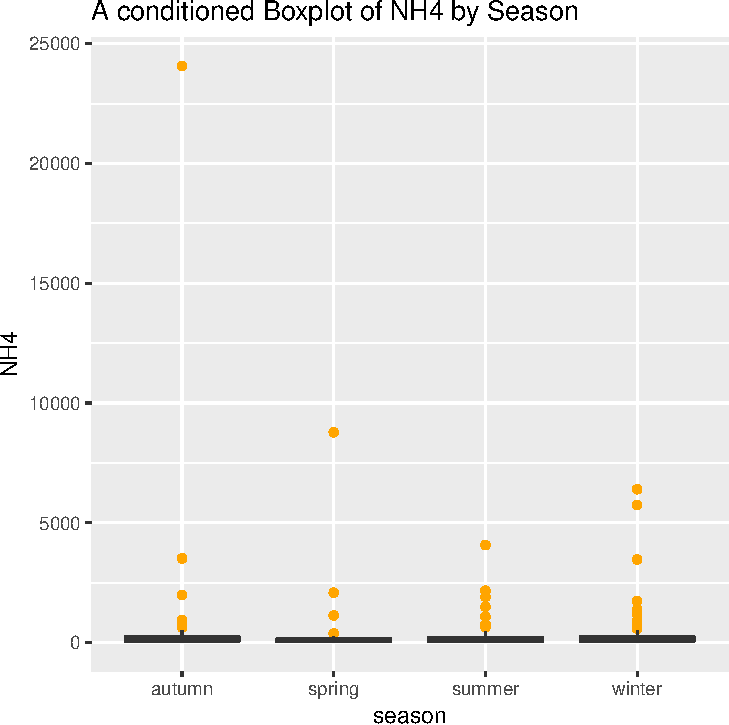
\includegraphics{homework1-handout_files/figure-latex/unnamed-chunk-3-2} \end{center}

\begin{enumerate}
\tightlist
\item
  Compare mean \& variance vs.~median \& MAD for \(NO3\) and \(NH4\).
  What do you notice? Can you conclude which set of measures is more
  robust when outliers are present?
\end{enumerate}

There is a larger difference between mean and median values for NH4 than
NO3. The same pattern is true for variance and MAD, however the variance
is much larger for NH4 than NO3. The median and MAD are a more
appropriate measure when outliers are present because the value in
autumn seems to skew our data when considered in parameters that average
all values.

\begin{center}\rule{0.5\linewidth}{\linethickness}\end{center}

\textbf{Predicting Algae Blooms}

Some water samples contained unknown values in several chemicals.
Missing data are very common in real-world problems, and may prevent the
use of certain data mining techniques that are not able to handle
missing values.

In this homework, we are going to introduce various ways to deal with
missing values. After all the missing values have been taken care of, we
will build a model to investigate the relationship between the variable
\texttt{a1} and other 11 predictors (\texttt{season}, \texttt{size},
\texttt{speed}, \texttt{mxPH}, \texttt{mnO2}, \texttt{Cl}, \texttt{NO3},
\texttt{NH4}, \texttt{oPO4}, \texttt{PO4}, \texttt{Chla}) utilizing
cross-validation in the next problem.

\textbf{\emph{Dealing with missing values}}

\begin{enumerate}
\def\labelenumi{\arabic{enumi}.}
\setcounter{enumi}{2}
\item
  \begin{enumerate}
  \tightlist
  \item
    How many observations contain missing values? How many missing
    values are there in each variable?
  \end{enumerate}
\end{enumerate}

\begin{Shaded}
\begin{Highlighting}[]
\NormalTok{missingvalues <-}\StringTok{ }\NormalTok{algae }\OperatorTok
\StringTok{  }\KeywordTok{select}\NormalTok{(}\KeywordTok{c}\NormalTok{(}\StringTok{'season'}\NormalTok{,}\StringTok{'size'}\NormalTok{,}\StringTok{'speed'}\NormalTok{,}\StringTok{'mxPH'}\NormalTok{,}\StringTok{'mnO2'}\NormalTok{,}\StringTok{'Cl'}\NormalTok{,}\StringTok{'NO3'}\NormalTok{,}\StringTok{'NH4'}\NormalTok{,}
  \StringTok{'oPO4'}\NormalTok{,}\StringTok{'PO4'}\NormalTok{,}\StringTok{'Chla'}\NormalTok{,}\StringTok{'a1'}\NormalTok{,}\StringTok{'a2'}\NormalTok{,}\StringTok{'a3'}\NormalTok{,}\StringTok{'a4'}\NormalTok{,}\StringTok{'a5'}\NormalTok{, }\StringTok{'a6'}\NormalTok{, }\StringTok{'a7'}\NormalTok{)) }\OperatorTok
\StringTok{  }\KeywordTok{summarise_all}\NormalTok{(}\ControlFlowTok{function}\NormalTok{(x) }\KeywordTok{sum}\NormalTok{(}\KeywordTok{is.na}\NormalTok{(x)))}

\KeywordTok{sum}\NormalTok{(missingvalues}\OperatorTok{>}\DecValTok{0}\NormalTok{)}
\end{Highlighting}
\end{Shaded}

\begin{verbatim}
## [1] 8
\end{verbatim}

There are 8 observations that contain missing values.

\begin{verbatim}
#. **Removing observations with missing values**: use `filter()` function
in `dplyr` package to observations with any missing value, and save the
resulting dataset (without missing values) as `algae.del`. Report how many
observations are in `algae.del`.

    Hint: `complete.cases()` may be useful.
\end{verbatim}

\begin{Shaded}
\begin{Highlighting}[]
\NormalTok{algae.del <-}\StringTok{ }\NormalTok{algae }\OperatorTok\StringTok{ }
\StringTok{  }\KeywordTok{filter_all}\NormalTok{(}\KeywordTok{all_vars}\NormalTok{(}\OperatorTok{!}\KeywordTok{is.na}\NormalTok{(.)))}
\end{Highlighting}
\end{Shaded}

\begin{verbatim}
#. \label{imputation} **Imputing unknowns with measures of central
tendency**: the simplest and fastest way of filling in (imputing) missing
values is to use some measures of central tendency such as mean, median and
mode.
    
    Use `mutate_at()` and `ifelse()` in `dplyr` to fill in missing values
    for each chemical with its median, and save the imputed dataset as
    `algae.med`. Report the number of observations in `algae.med`.  Display
    the values of each chemical for the $48^{th}$, $62^{th}$ and $199^{th}$
    obsevation in `algae.med`. 
\end{verbatim}

\begin{Shaded}
\begin{Highlighting}[]
\NormalTok{algae.med <-}\StringTok{ }\NormalTok{algae }\OperatorTok\StringTok{ }
\StringTok{  }\KeywordTok{mutate_at}\NormalTok{(}\DataTypeTok{.vars =} \KeywordTok{c}\NormalTok{(}\StringTok{'mxPH'}\NormalTok{,}\StringTok{'mnO2'}\NormalTok{,}\StringTok{'Cl'}\NormalTok{,}\StringTok{'NO3'}\NormalTok{,}\StringTok{'NH4'}\NormalTok{,}
  \StringTok{'oPO4'}\NormalTok{,}\StringTok{'PO4'}\NormalTok{,}\StringTok{'Chla'}\NormalTok{), }\DataTypeTok{.funs =} \KeywordTok{funs}\NormalTok{(}\KeywordTok{ifelse}\NormalTok{(}\KeywordTok{is.na}\NormalTok{(.), }\KeywordTok{median}\NormalTok{(., }\DataTypeTok{na.rm =} \OtherTok{TRUE}\NormalTok{), .)))}

\NormalTok{algae.med.}\DecValTok{48}\NormalTok{ <-}\StringTok{ }\NormalTok{algae.med[}\DecValTok{48}\NormalTok{, }\DecValTok{4}\OperatorTok{:}\DecValTok{11}\NormalTok{]}
\NormalTok{algae.med.}\DecValTok{62}\NormalTok{ <-}\StringTok{ }\NormalTok{algae.med[}\DecValTok{62}\NormalTok{, }\DecValTok{4}\OperatorTok{:}\DecValTok{11}\NormalTok{]}
\NormalTok{algae.med.}\DecValTok{199}\NormalTok{ <-}\StringTok{ }\NormalTok{algae.med[}\DecValTok{199}\NormalTok{, }\DecValTok{4}\OperatorTok{:}\DecValTok{11}\NormalTok{]}

\NormalTok{algae.med.rows <-}\StringTok{ }\KeywordTok{rbind}\NormalTok{(algae.med.}\DecValTok{48}\NormalTok{, algae.med.}\DecValTok{62}\NormalTok{, algae.med.}\DecValTok{199}\NormalTok{)}
\KeywordTok{rownames}\NormalTok{(algae.med.rows) <-}\StringTok{ }\KeywordTok{c}\NormalTok{(}\StringTok{"48"}\NormalTok{, }\StringTok{"62"}\NormalTok{, }\StringTok{"199"}\NormalTok{)}
\end{Highlighting}
\end{Shaded}

\begin{verbatim}
## Warning: Setting row names on a tibble is deprecated.
\end{verbatim}

\begin{Shaded}
\begin{Highlighting}[]
\KeywordTok{kable}\NormalTok{(algae.med.rows, }\StringTok{"latex"}\NormalTok{, }\DataTypeTok{booktabs =}\NormalTok{ T, }
      \DataTypeTok{caption =} \StringTok{"Chemical Observations for Specific Rows After Imputing"}\NormalTok{) }\OperatorTok\StringTok{  }
\StringTok{      }\KeywordTok{kable_styling}\NormalTok{(}\DataTypeTok{bootstrap_options =} \StringTok{"striped"}\NormalTok{, }\DataTypeTok{full_width =}\NormalTok{ F, }\DataTypeTok{position =} \StringTok{"center"}\NormalTok{)}
\end{Highlighting}
\end{Shaded}

\begin{table}

\caption{\label{tab:unnamed-chunk-5}Chemical Observations for Specific Rows After Imputing}
\centering
\begin{tabular}[t]{lrrrrrrrr}
\toprule
  & mxPH & mnO2 & Cl & NO3 & NH4 & oPO4 & PO4 & Chla\\
\midrule
48 & 8.06 & 12.6 & 9.00 & 0.230 & 10.0000 & 5.00 & 6.0000 & 1.100\\
62 & 6.40 & 9.8 & 32.73 & 2.675 & 103.1665 & 40.15 & 14.0000 & 5.475\\
199 & 8.00 & 7.6 & 32.73 & 2.675 & 103.1665 & 40.15 & 103.2855 & 5.475\\
\bottomrule
\end{tabular}
\end{table}

There are 200 observations in algae.med.

\begin{verbatim}
    This simple strategy, although extremely fast and thus appealing for
    large datasets, imputed values may have large bias that can influence
    our model fitting. An alternative for decreasing bias of imputed values
    is to use relationships between variables.
    
#. **Imputing unknowns using correlations**: another way to impute missing
values is to use correlation with another variable. For a highly
correlated pair of variables, we can fill in the unknown values by
predicting one based on the other with a simple linear regression model,
provided the two variables are not both unknown. 

    Compute pairwise correlation between the continuous (chemical) variables. 




    Then, fill in the missing value for `PO4` based on `oPO4` in the
    $28^{th}$ observation. What is the value you obtain? 
    
    Hint: use `lm()` and `predict()` function.


#. **Questioning missing data assumptions**:  When might imputation using only the observed data lead you to incorrect conclusions?  In a couple of sentences, describe a scenario in which the imputed values of the chemical abundances in the algae data  (imputed using either the median or correlation method) might be a poor substitute for the true missing values.  Hint: look at the example from lecture 2.  
\end{verbatim}

\textbf{\emph{Estimating the Test Error with Cross Validation (CV)}}

Using \texttt{algae.med} dataset obtained in \eqref{imputation}, we will
build a linear regression model to predict the levels of algae type
\texttt{a1} based on 11 variables (\texttt{season}, \texttt{size},
\texttt{speed}, \texttt{mxPH}, \texttt{mnO2}, \texttt{Cl}, \texttt{NO3},
\texttt{NH4}, \texttt{oPO4}, \texttt{PO4}, \texttt{Chla}), and test
generalization of model to data that have not been used for training.

\begin{enumerate}
\def\labelenumi{\arabic{enumi}.}
\setcounter{enumi}{3}
\item
  \textbf{Cross-validation}: in class we talked about how to use
  cross-validation (CV) to estimate the ``test error''. In \(k\)-fold
  CV, each of \(k\) equally sized random˜ partitions of data (chunks)
  are used in a heldout set (called validation set or test set). After
  \(k\) runs, we average the held-out error as our final estimate of the
  validation error. For this part, we will run cross-validation on only
  a single model, as a way to estimate our test error for future
  predictions (we are not using it here for model selection since we are
  considering only one model). Perform 5-fold cross-validation on this
  model to estimate the (average) test error.

  \begin{enumerate}
  \item
    \label{chunkids} First randomly partition data into 5 equal sized
    chunks.

    Hint: a simple way to randomly assign each observation to a chunk is
    to do the following. First, use \texttt{cut(...,\ label=FALSE)} to
    divide observation ids (1, 2, \dots ) into equal numbers of chunk
    ids. Then, randomize output of \texttt{cut()}by using
    \texttt{sample()}.
  \item
    Perform 5-fold cross-validation with training error and validation
    errors of each chunk determined from \eqref{chunkids}.

    Since same computation is repeated 5 times, we can define the
    following function for simplicity.

\begin{Shaded}
\begin{Highlighting}[]
\NormalTok{do.chunk <-}\StringTok{ }\ControlFlowTok{function}\NormalTok{(chunkid, chunkdef, dat)\{  }\CommentTok{# function argument}

\NormalTok{    train =}\StringTok{ }\NormalTok{(chunkdef }\OperatorTok{!=}\StringTok{ }\NormalTok{chunkid)}

\NormalTok{    Xtr =}\StringTok{ }\NormalTok{dat[train,}\DecValTok{1}\OperatorTok{:}\DecValTok{11}\NormalTok{]  }\CommentTok{# get training set}
\NormalTok{    Ytr =}\StringTok{ }\NormalTok{dat[train,}\DecValTok{12}\NormalTok{]  }\CommentTok{# get true response values in trainig set}

\NormalTok{    Xvl =}\StringTok{ }\NormalTok{dat[}\OperatorTok{!}\NormalTok{train,}\DecValTok{1}\OperatorTok{:}\DecValTok{11}\NormalTok{]  }\CommentTok{# get validation set}
\NormalTok{    Yvl =}\StringTok{ }\NormalTok{dat[}\OperatorTok{!}\NormalTok{train,}\DecValTok{12}\NormalTok{]  }\CommentTok{# get true response values in validation set}

\NormalTok{    lm.a1 <-}\StringTok{ }\KeywordTok{lm}\NormalTok{(a1}\OperatorTok{~}\NormalTok{., }\DataTypeTok{data =}\NormalTok{ dat[train,}\DecValTok{1}\OperatorTok{:}\DecValTok{12}\NormalTok{])}
\NormalTok{    predYtr =}\StringTok{ }\KeywordTok{predict}\NormalTok{(lm.a1)  }\CommentTok{# predict training values}
\NormalTok{    predYvl =}\StringTok{ }\KeywordTok{predict}\NormalTok{(lm.a1,Xvl)  }\CommentTok{# predict validation values}

    \KeywordTok{data.frame}\NormalTok{(}\DataTypeTok{fold =}\NormalTok{ chunkid,}
               \DataTypeTok{train.error =} \KeywordTok{mean}\NormalTok{((predYtr }\OperatorTok{-}\StringTok{ }\NormalTok{Ytr)}\OperatorTok{^}\DecValTok{2}\NormalTok{), }\CommentTok{# compute and store training error}
               \DataTypeTok{val.error =} \KeywordTok{mean}\NormalTok{((predYvl }\OperatorTok{-}\StringTok{ }\NormalTok{Yvl)}\OperatorTok{^}\DecValTok{2}\NormalTok{))   }\CommentTok{# compute and store test error}

\NormalTok{\}}
\end{Highlighting}
\end{Shaded}

    First argument \texttt{chunkid} indicates which chunk to use as
    validation set (one of 1:5). Second argument \texttt{chunkdef} is
    chunk assignments from \eqref{chunkids}. Third argument \texttt{dat}
    will be \texttt{algae.med} dataset.

    In order to repeatedly call \texttt{do.chunk()} for each value of
    \texttt{chunkid}, use functions \texttt{lapply()} or
    \texttt{ldply()}. Note that \texttt{chunkdef} and \texttt{dat}
    should be passed in as optional arguments (refer to help pages).

    Write the code and print out the \texttt{train.error} and
    \texttt{val.error} five times (e.g.~for each chunk).
  \end{enumerate}
\item
  \textbf{Test error on additional data}: now imagine that you actually
  get \emph{new} data that wasn't available when you first fit the
  model.

  \begin{enumerate}
  \item
    Additional data can be found in the file \texttt{algaeTest.txt}.

\begin{Shaded}
\begin{Highlighting}[]
\NormalTok{algae.Test <-}\StringTok{ }\KeywordTok{read_table2}\NormalTok{(}\StringTok{'algaeTest.txt'}\NormalTok{,}
                    \DataTypeTok{col_names=}\KeywordTok{c}\NormalTok{(}\StringTok{'season'}\NormalTok{,}\StringTok{'size'}\NormalTok{,}\StringTok{'speed'}\NormalTok{,}\StringTok{'mxPH'}\NormalTok{,}\StringTok{'mnO2'}\NormalTok{,}\StringTok{'Cl'}\NormalTok{,}\StringTok{'NO3'}\NormalTok{,}
                                \StringTok{'NH4'}\NormalTok{,}\StringTok{'oPO4'}\NormalTok{,}\StringTok{'PO4'}\NormalTok{,}\StringTok{'Chla'}\NormalTok{,}\StringTok{'a1'}\NormalTok{),}
                    \DataTypeTok{na=}\KeywordTok{c}\NormalTok{(}\StringTok{'XXXXXXX'}\NormalTok{))}
\end{Highlighting}
\end{Shaded}

    This data was not used to train the model and was not (e.g.~wasn't
    used in the CV procedure to estimate the test error). We can get a
    more accurate measure of true test error by evaluating the model fit
    on this held out set of data. Using the same linear regression model
    from part 4 (fit to all of the training data), calculate the
    ``true'' test error of your predictions based on the newly collected
    measurements in \texttt{algaeTest.txt}. Is this roughly what you
    expected based on the CV estimated test error from part 4?
  \end{enumerate}
\end{enumerate}

\textbf{\emph{Cross Validation (CV) for Model Selection}}

In this problem, we will be exploring a dataset of wages from a group of
3000 workers. The goal in this part is to identify a relationship
between wages and age.

\begin{enumerate}
\def\labelenumi{\arabic{enumi}.}
\setcounter{enumi}{5}
\item
  First, install the \texttt{ISLR} package, which includes many of the
  datasets used in the ISLR textbook. Look at the variables defined in
  the \texttt{Wage} dataset. We will be using the \texttt{wage} and
  \texttt{age} variables for this problem.

\begin{Shaded}
\begin{Highlighting}[]
\KeywordTok{library}\NormalTok{(ISLR)}
\KeywordTok{head}\NormalTok{(Wage)}
\end{Highlighting}
\end{Shaded}

  \begin{enumerate}
  \item
    Plot wages as a function of age using \texttt{ggplot}. Your plot
    should include the datapoints (\texttt{geom\_point()}) as well as a
    smooth fit to the data (\texttt{geom\_smooth()}). Based on your
    visualization, what is the general pattern of wages as a function of
    age? Does this match what you expect?
  \item
    In this part of the problem, we will find a polynomial function of
    age that best fits the wage data. For each polynomial function
    between \(p=0, 1, 2, ... 10\):

    \begin{enumerate}
    \tightlist
    \item
      Fit a linear regression to predict wages as a function of \(age\),
      \(age^2\), \ldots{} \(age^p\) (you should include an intercept as
      well). Note that \(p=0\) model is an ``intercept-only'' model.
    \item
      Use 5-fold cross validation to estimate the test error for this
      model. Save both the test error and the training error.
    \end{enumerate}
  \item
    Plot both the test error and training error (on the same plot) for
    each of the models estimated above as a function of \(p\). What do
    you observe about the training error as \(p\) increases? What about
    the test error? Based on your results, which model should you select
    and why?
  \end{enumerate}

  Note: \texttt{poly(age,\ degree=p,\ raw=TRUE)} will return a matrix
  with \(p\) columns, where the \(p\)-th column is \(age^p\). For the
  predictors in your regression use
  \texttt{poly(age,\ degree=p,\ raw=FALSE)}. The \texttt{raw=FALSE}
  option returns predictors which are numerically more stable (it
  returns a matrix of ``orthogonal polynomials''). Numerical stability
  can be an issue because \(age^p\) can be very very large if \(p\) is
  large. The orthogonal polynomials returned when \texttt{raw=FALSE} are
  rescaled to account for this so please use the \texttt{raw=FALSE}
  option.\\
  Hint: A function similar to \texttt{do.chunk} from problem 4 will be
  helpful here as well.
\end{enumerate}

\begin{center}\rule{0.5\linewidth}{\linethickness}\end{center}

\begin{enumerate}
\def\labelenumi{\arabic{enumi}.}
\setcounter{enumi}{6}
\item
  \textbf{(231 Only)} \textbf{The bias-variance tradeoff}. Prove that
  the mean squared error can be decomposed into the variance plus bias
  squared. That is, who
  \(E[(\hat \theta - \theta)^2] = \text{Var}(\hat \theta) + \text{Bias}(\hat \theta )^2\)
  where \(\text{Bias}(\hat \theta) = E[\hat \theta - \theta]\). Here
  \(\hat \theta\) is an estimator (a random variable) of the fixed
  unknown constant \(\theta\). Hint: reogranize terms in the MSE by
  adding and subtracting \(E[\hat \theta]\).
\item
  \textbf{(231 Only)} As we discussed in class, distance metrics satisfy
  the following properties:

  \begin{itemize}
  \item
    \emph{Positivity}:

    \begin{itemize}
    \tightlist
    \item
      \(d(x,y)\geq 0\)
    \item
      \(d(x,y) = 0\) only if \(x=y\)
    \end{itemize}
  \item
    \emph{Symmetry}:

    \begin{itemize}
    \tightlist
    \item
      \(d(x,y) = d(y,x)\) for all \(x\) and \(y\)
    \end{itemize}
  \item
    \emph{Triangle Inequality}:

    \begin{itemize}
    \tightlist
    \item
      \(d(x,z) \leq d(x,y) + d(y,z)\) for \(x,\ y,\text{ and } z\)
    \end{itemize}
  \end{itemize}

  Show that the following measures are distance metrics by showing the
  above properties hold:

  \begin{enumerate}
  \item
    \(d(x,y) = \|x-y\|_2\)
  \item
    \(d(x,y) = \|x-y\|_\infty\)
  \end{enumerate}
\end{enumerate}


\end{document}
